\documentclass[tikz,border=5pt]{standalone}
\usepackage{amsmath}
\usetikzlibrary{arrows,calc}

\definecolor{dataBlue}{HTML}{4C78A8}
\definecolor{baselineGray}{HTML}{8C8C8C}
\definecolor{residualAmber}{HTML}{E08E2B}
\definecolor{correctionTeal}{HTML}{2A9D8F}
\definecolor{predictionGreen}{HTML}{59A14F}
\definecolor{charcoal}{HTML}{3A3A3A}

\newcommand{\modulelabel}[1]{%
  {\sffamily\fontsize{10}{12}\selectfont\bfseries #1}%
}

\begin{document}
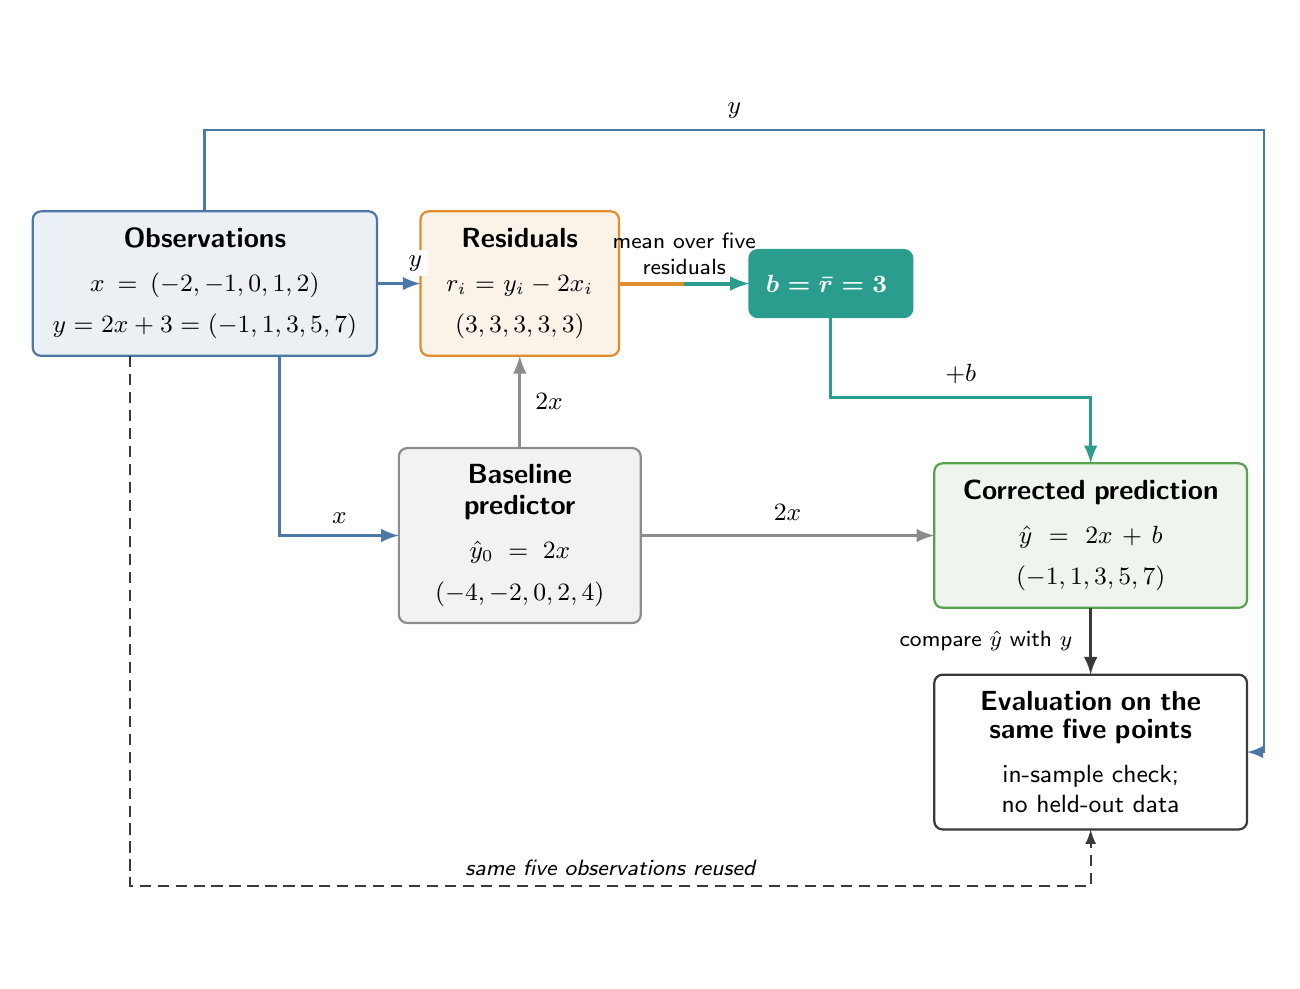
\begin{tikzpicture}[
  font=\fontsize{9}{11}\selectfont,
  block/.style={
    rectangle,
    rounded corners=3pt,
    line width=0.8pt,
    inner xsep=6pt,
    inner ysep=6pt,
    outer sep=0pt,
    align=center
  },
  flow/.style={
    -latex,
    line width=1.2pt,
    draw=charcoal
  },
  mathlabel/.style={
    font=\fontsize{9}{11}\selectfont,
    inner sep=2pt,
    fill=white
  },
  smalllabel/.style={
    font=\sffamily\fontsize{8}{9.5}\selectfont,
    inner sep=2pt,
    fill=white,
    align=center
  }
]

% White canvas with the requested 4:3 aspect ratio.
\path[use as bounding box] (0,0) rectangle (15.8,11.85);
\fill[white] (0,0) rectangle (15.8,11.85);

% Column 1: observations.
\node[
  block,
  draw=dataBlue,
  fill=dataBlue!11!white,
  text width=3.95cm,
  minimum height=1.8cm
] (D) at (2.25,8.6) {%
  \modulelabel{Observations}\\[5pt]
  $x=(-2,-1,0,1,2)$\\[4pt]
  $y=2x+3=(-1,1,3,5,7)$
};

% Column 2: residuals and baseline.
\node[
  block,
  draw=residualAmber,
  fill=residualAmber!11!white,
  text width=2.1cm,
  minimum height=1.8cm
] (R) at (6.25,8.6) {%
  \modulelabel{Residuals}\\[5pt]
  $r_i=y_i-2x_i$\\[4pt]
  $(3,3,3,3,3)$
};

\node[
  block,
  draw=baselineGray,
  fill=baselineGray!11!white,
  text width=2.65cm,
  minimum height=1.8cm
] (B) at (6.25,5.4) {%
  \modulelabel{Baseline predictor}\\[5pt]
  $\hat{y}_0=2x$\\[4pt]
  $(-4,-2,0,2,4)$
};

% Column 3: scalar correction.
\node[
  block,
  draw=correctionTeal,
  fill=correctionTeal,
  text=white,
  minimum width=1.7cm,
  minimum height=0.85cm
] (S) at (10.2,8.6) {%
  $\boldsymbol{b=\bar{r}=3}$
};

% Column 4: corrected prediction and evaluation.
\node[
  block,
  draw=predictionGreen,
  fill=predictionGreen!11!white,
  text width=3.55cm,
  minimum height=1.8cm
] (C) at (13.5,5.4) {%
  \modulelabel{Corrected prediction}\\[5pt]
  $\hat{y}=2x+b$\\[4pt]
  $(-1,1,3,5,7)$
};

\node[
  block,
  draw=charcoal,
  fill=white,
  text width=3.55cm,
  minimum height=1.85cm
] (E) at (13.5,2.65) {%
  \modulelabel{Evaluation on the}\\[-1pt]
  \modulelabel{same five points}\\[5pt]
  {\sffamily\fontsize{9}{11}\selectfont
   in-sample check;\\
   no held-out data}
};

% Observed targets enter the residual calculation directly.
\draw[flow,draw=dataBlue]
  (D.east) -- (R.west)
  node[mathlabel,pos=0.88,above=2pt] {$y$};

% Inputs branch downward and then right into the baseline.
\coordinate (inputExit) at ($(D.south)+(0.95,0)$);
\draw[flow,draw=dataBlue]
  (inputExit) |- (B.west);
\node[mathlabel,above=2pt]
  at ($(inputExit |- B.west)!0.5!(B.west)$) {$x$};

% Baseline predictions enter the residual calculation vertically.
\draw[flow,draw=baselineGray]
  (B.north) -- (R.south)
  node[mathlabel,midway,right=3pt] {$2x$};

% Mean residual: a continuous amber-to-teal connector.
\coordinate (meanMid) at ($(R.east)!0.5!(S.west)$);
\draw[draw=residualAmber,line width=1.4pt]
  (R.east) -- (meanMid);
\draw[-latex,draw=correctionTeal,line width=1.4pt]
  (meanMid) -- (S.west);
\node[
  font=\sffamily\fontsize{8}{9.5}\selectfont,
  align=center,
  inner sep=0pt,
  anchor=south
] at ($(meanMid)+(0,3pt)$) {mean over five\\residuals};

% Baseline contribution to the corrected prediction.
\draw[flow,draw=baselineGray]
  (B.east) -- (C.west)
  node[mathlabel,midway,above=3pt] {$2x$};

% Scalar correction steps down and right into the prediction.
\draw[flow,draw=correctionTeal]
  (S.south)
  -- (10.2,7.15)
  -- (13.5,7.15)
  -- (C.north);
\node[mathlabel,above=3pt] at (11.85,7.15) {$+b$};

% Corrected predictions are evaluated on the original targets.
\draw[flow]
  (C.south) -- (E.north)
  node[smalllabel,midway,left=4pt]
  {compare $\hat{y}$ with $y$};

% Target reuse: solid blue perimeter route into evaluation's right flank.
\draw[-latex,draw=dataBlue,line width=1.0pt]
  (D.north)
  -- (2.25,10.55)
  -- (15.7,10.55)
  -- (15.7,2.65)
  -- (E.east);
\node[mathlabel,above=2pt] at (8.975,10.55) {$y$};

% Explicit provenance of the reused observations.
\coordinate (reuseExit) at ($(D.south)+(-0.95,0)$);
\draw[
  -latex,
  draw=charcoal,
  line width=0.8pt,
  dash pattern=on 4pt off 2.5pt
]
  (reuseExit)
  -- (1.3,0.95)
  -- (13.5,0.95)
  -- (E.south);
\node[
  font=\sffamily\fontsize{8}{9.5}\selectfont\itshape,
  fill=white,
  inner sep=1pt,
  anchor=south
] at (7.4,1.04) {same five observations reused};

\end{tikzpicture}
\end{document}